\documentclass{article}
\usepackage[UKenglish]{babel}
\usepackage[UKenglish]{isodate}
\usepackage{enumerate}
\usepackage[a4paper, inner=2cm, outer=2cm, top=2cm, bottom=2cm, bindingoffset=0cm]{geometry}
\usepackage{fancyhdr}
\usepackage{graphicx}
\usepackage{amsmath}

\def\cramersMatrix#1#2#3#4#5#6#7#8#9{
  \def\a{{#1}}
  \def\b{{#2}}
  \def\c{{#3}}
  \def\d{{#4}}
  \def\e{{#5}}
  \def\f{{#6}}
  \def\g{{#7}}
  \def\h{{#8}}
  \def\i{{#9}}
}

\def\cramersVector#1#2#3{
  \def\j{{#1}}
  \def\k{{#2}}
  \def\l{{#3}}
}

\newcommand{\cramers}[0]
{
\[
	\left(
		\begin{array}{ccc}
			\a & \b & \c \\
			\d & \e & \f \\
			\g & \h & \i
		\end{array}
	\right)
	\left(
		\begin{array}{c}
			x \\
			y \\
			z
		\end{array}
	\right)
	=
	\left(
		\begin{array}{c}
			\j \\
			\k \\
			\l
		\end{array}
	\right)
	\Rightarrow
	x=
	\frac
	{
		\left|
			\begin{array}{ccc}
				\j & \b & \c \\
				\k & \e & \f \\
				\l & \h & \i
			\end{array}
		\right|
	}
	{
		\left|
			\begin{array}{ccc}
				\a & \b & \c \\
				\d & \e & \f \\
				\g & \h & \i
			\end{array}
		\right|
	},
	y=
	\frac
	{
		\left|
			\begin{array}{ccc}
				\a & \j & \c \\
				\d & \k & \f \\
				\g & \l & \i
			\end{array}
		\right|
	}
	{
		\left|
			\begin{array}{ccc}
				\a & \b & \c \\
				\d & \e & \f \\
				\g & \h & \i
			\end{array}
		\right|
	},
	z=
	\frac
	{
		\left|
			\begin{array}{ccc}
				\a & \b & \j \\
				\d & \e & \k \\
				\g & \h & \l
			\end{array}
		\right|
	}
	{
		\left|
			\begin{array}{ccc}
				\a & \b & \c \\
				\d & \e & \f \\
				\g & \h & \i
			\end{array}
		\right|
	}
\]
}

\newcommand{\determinant}[9]
{
\cramersMatrix{#1}{#2}{#3}{#4}{#5}{#6}{#7}{#8}{#9}
\[
	\left|
		\begin{array}{ccc}
			\a & \b & \c \\
			\d & \e & \f \\
			\g & \h & \i
		\end{array}
	\right|
	= (\a \cdot \e \cdot \i) - (\a \cdot \h \cdot \f) - (\b \cdot \d \cdot \i) + (\b \cdot \g \cdot \f) + (\c \cdot \d \cdot \h) - (\c \cdot \e \cdot \g)
\]
}

\pagestyle{fancy}
\lhead{Portfolio Excerise: Mathematics and Modelling for Games}
\rhead{Antony Bartlett}
\begin{document}
\title{Portfolio Excerise: Mathematics and Modelling for Games}
\author{Antony Bartlett}
\maketitle
\begin{enumerate}

% Question 1
\item

\begin{enumerate}[i.]

% Part i
\item The distance between the two points is
\[
\sqrt{ (a-c)^2 + (b-d)^2 }
\]
\\

% Part ii
\item A line can be described by the equation
\[
y=mx+c
\]

Put the gradient in
\[
y=\frac{d-b}{c-a}x+c
\]

At the point (a,b)
\[
b=\frac{d-b}{c-a}a + c
\]

Thus
\[
c=b - \frac{d-b}{c-a}a
\]

Hence the equation of the line is
\[
y=\frac{d-b}{c-a}x+b - \frac{d-b}{c-a}a
\]

Which simplifies to
\[
y=\frac{(d-b)(x-a)}{c-a} + b
\]
\\

% Part iii
\item The mid-point of the two points is
\[
(\frac{a+c}{2}, \frac{b+d}{2})
\]
\\

% Part iv
\item The gradient of the line joining the two points is
\[
\frac{d-b}{c-a}
\]
\\

% Part v
\item The gradient of the normal is
\[
\frac{a-c}{d-b}
\]
\\

% Part vi
\item The gradient of the tangent joining the two points is
\[
\frac{d-b}{c-a}
\]
\\

\end{enumerate}

% Question 2
\item Cramer's rule (3x3):
\cramersMatrix{a}{b}{c}{d}{e}{f}{g}{h}{i}
\cramersVector{j}{k}{l}
\cramers

Determinants (3x3):
\[
	\left|
		\begin{array}{cc}
			a & b \\
			c & d
		\end{array}
	\right|
	= ad - bc
\]
\[
	\left|
		\begin{array}{ccc}
			a & b & c \\
			d & e & f \\
			g & h & i
		\end{array}
	\right|
	=a
	\left|
		\begin{array}{cc}
			e & f \\
			h & i
		\end{array}
	\right|
	-b
	\left|
		\begin{array}{cc}
			d & f \\
			g & i
		\end{array}
	\right|
	+c
	\left|
		\begin{array}{cc}
			d & e \\
			g & h
		\end{array}
	\right|
	= aei - ahf - bdi + bgf + cdh - ceg
\]

Since determinants are being calculating anyway, this method of matrix inversion will be used:
\[
	\left(
		\begin{array}{ccc}
			a & b & c \\
			d & e & f \\
			g & h & i
		\end{array}
	\right)^{-1}
	=
	\frac{1}
	{
		\left|
			\begin{array}{ccc}
				a & b & c \\
				d & e & f \\
				g & h & i
			\end{array}
		\right|
	}
	\left(
		\begin{array}{ccc}
			ei-fh & ch-bi & bf-ce \\
			fg-di & ai-cg & cd-af \\
			dh-eg & bg-ah & ae-bd
		\end{array}
	\right)
\]

\begin{enumerate}[i.]

% Part i
\item
\cramersMatrix{2}{3}{7}{3}{5}{1}{3}{4}{{^-}2}
\cramersVector{12}{9}{5}
\cramers

\determinant{2}{3}{7}{3}{5}{1}{3}{4}{{^-}2}
\[
	= {^-}20 - 8 - {^-}18 + 9 + 84 - 105 = {^-}22
\]

\determinant{12}{3}{7}{9}{5}{1}{5}{4}{{^-}2}
\[
	= {^-}120 - 48 - {^-}54 + 15 + 252 - 175 = {^-}22
\]

\determinant{2}{12}{7}{3}{9}{1}{3}{5}{{^-}2}
\[
	= {^-}36 - 10 - {^-}72 + 36 + 105 - 189 = {^-}22
\]

\determinant{2}{3}{12}{3}{5}{9}{3}{4}{5}
\[
	= 50 - 72 - 45 + 81 + 144 - 180 = {^-}22
\]

Therefore
\[
	\left(
		\begin{array}{c}
			x \\
			y \\
			z
		\end{array}
	\right)
	=
	\left(
		\begin{array}{c}
			\frac{{^-}22}{{^-}22} \\
			\frac{{^-}22}{{^-}22} \\
			\frac{{^-}22}{{^-}22}
		\end{array}
	\right)
	=
	\left(
		\begin{array}{c}
			1 \\
			1 \\
			1
		\end{array}
	\right)
\]

Now invert the matrix
\[
	\left(
		\begin{array}{ccc}
			2 & 3 & 7 \\
			3 & 5 & 1 \\
			3 & 4 & {^-}2
		\end{array}
	\right)^{-1}
	=
	\frac{1}{-22}
	\left(
		\begin{array}{ccc}
			(5 \cdot {^-}2)-(1 \cdot 4) & (7 \cdot 4)-(3 \cdot {^-}2) & (3 \cdot 1)-(7 \cdot 5) \\
			(1 \cdot 3)-(3 \cdot {^-}2) & (2 \cdot {^-}2)-(7 \cdot 3) & (7 \cdot 3)-(2 \cdot 1) \\
			(3 \cdot 4)-(5 \cdot 3)        & (3 \cdot 3)-(2 \cdot 4)         & (2 \cdot 5)-(3 \cdot 3)
		\end{array}
	\right)
	=
	-\frac{1}{22}
	\left(
		\begin{array}{ccc}
		 {^-}14 &          34 &  {^-}32 \\
		           9 &  {^-}25 &         19  \\
 		    {^-}3 &           1 &           1
		\end{array}	
	\right)
\]

So
\[
	\left(
		\begin{array}{c}
			x \\
			y \\
			z
		\end{array}
	\right)
	=
	-\frac{1}{22}
	\left(
		\begin{array}{ccc}
		 {^-}14 &          34 &  {^-}32 \\
		           9 &  {^-}25 &         19  \\
 		    {^-}3 &           1 &           1
		\end{array}	
	\right)
	\left(
		\begin{array}{c}
			12 \\
			9 \\
			5
		\end{array}
	\right)
	=
	-\frac{1}{22}
	\left(
		\begin{array}{c}
			 {^-}14 \cdot 12 +        34 \cdot 9 +  {^-}32 \cdot5 \\
			          9 \cdot 12 + {^-}25 \cdot 9 +         19 \cdot 5 \\
			   {^-}3 \cdot 12 +          1 \cdot 9 +           1 \cdot 5
		\end{array}
	\right)
\]
\[
	=
	-\frac{1}{22}
	\left(
		\begin{array}{c}
			 {^-}168 + 306 - 160 \\
			         108 -  225 + 95 \\
			   {^-} 36+     9 +   5
		\end{array}
	\right)
	=
	-\frac{1}{22}
	\left(
		\begin{array}{c}
			 -22 \\
			 -22 \\
			  -22
		\end{array}
	\right)
\]
Which confirms
\[
	\left(
		\begin{array}{c}
			x \\
			y \\
			z
		\end{array}
	\right)
	=
	\left(
		\begin{array}{c}
			1 \\
			1 \\
			1
		\end{array}
	\right)
\]
\\

% Question 2 part ii
\item
\cramersMatrix{{^-}2}{3}{4}{1}{{^-}2}{0}{0}{1}{1}
\cramersVector{1}{{^-}1}{2}
\cramers

\determinant{{^-}2}{3}{4}{1}{{^-}2}{0}{0}{1}{1}
\[
	= 4 - 0 - 3 + 0 + 4 + 0 = 5
\]

\determinant{1}{3}{4}{{^-}1}{{^-}2}{0}{2}{1}{1}
\[
	= -2 - 0 + 3 + 0 - 4 + 16 = 13
\]

\determinant{{^-}2}{1}{4}{1}{{^-}1}{0}{0}{2}{1}
\[
	= 2 + 0 - 1 + 0 + 8 + 0 = 9
\]

\determinant{{^-}2}{3}{1}{1}{{^-}2}{{^-}1}{0}{1}{2}
\[
	= 8 - 2 - 6 + 0 +1 + 0 = 1
\]

Therefore
\[
	\left(
		\begin{array}{c}
			x \\
			y \\
			z
		\end{array}
	\right)
	=
	\left(
		\begin{array}{c}
			\frac{13}{5} \\
			\frac{9}{5} \\
			\frac{1}{5}
		\end{array}
	\right)
	=
	\left(
		\begin{array}{c}
			2.6 \\
			1.8 \\
			0.2
		\end{array}
	\right)
\]

Now invert the matrix
\[
	\left(
		\begin{array}{ccc}
			{^-}2 &        3 & 4 \\
			       1 & {^-}2 & 0 \\
			       0 &        1 & 1
		\end{array}
	\right)^{-1}
	=
	\frac{1}{5}
	\left(
		\begin{array}{ccc}
			({^-}2 \cdot 1)-(0         \cdot 1) & (       4 \cdot 1)-(       3 \cdot 1) & (       3 \cdot         0)-({^-}2  \cdot 4) \\
			(       0  \cdot 0)-(1        \cdot 1) & ({^-}2 \cdot 1)-(       0 \cdot 4) & (       4 \cdot         1)-({^-}2 \cdot 0) \\
			(       1  \cdot 1)-({^-}2 \cdot 0) & (       3 \cdot 0)-({^-}2 \cdot 1) & ({^-}2 \cdot {^-}2)-(        3 \cdot 1)
		\end{array}
	\right)
	=
	\frac{1}{5}
	\left(
		\begin{array}{ccc}
			{^-}2 &        1 & 8 \\
			{^-}1 & {^-}2 & 4 \\
			1        &         2 & 1
		\end{array}	
	\right)
\]

So
\[
	\left(
		\begin{array}{c}
			x \\
			y \\
			z
		\end{array}
	\right)
	=
	\frac{1}{5}
	\left(
		\begin{array}{ccc}
			{^-}2 &        1 & 8 \\
			{^-}1 & {^-}2 & 4 \\
			1        &         2 & 1
		\end{array}	
	\right)
	\left(
		\begin{array}{c}
			       1 \\
			{^-}1 \\
			       2
		\end{array}
	\right)
	=
	\frac{1}{5}
	\left(
		\begin{array}{c}
			 {^-}2 \cdot 1 +        1 \cdot {^-}1 +  8 \cdot2 \\
			 {^-}1 \cdot 1 + {^-}2 \cdot {^-}1 +  4 \cdot 2 \\
			         1 \cdot 1 +        2 \cdot {^-}1 +  1 \cdot 2
		\end{array}
	\right)
\]
\[
	=
	\frac{1}{5}
	\left(
		\begin{array}{c}
			 -2 - 1 +16 \\
			 -1 + 2 + 8 \\
			 1 - 2 + 2
		\end{array}
	\right)
	=
	\frac{1}{5}
	\left(
		\begin{array}{c}
			 13 \\
			 9 \\
			 1
		\end{array}
	\right)
\]
Which confirms
\[
	\left(
		\begin{array}{c}
			x \\
			y \\
			z
		\end{array}
	\right)
	=
	\left(
		\begin{array}{c}
			\frac{13}{5} \\
			\frac{9}{5} \\
			\frac{1}{5}
		\end{array}
	\right)
	=
	\left(
		\begin{array}{c}
			2.6 \\
			1.8 \\
			0.2
		\end{array}
	\right)
\]
\\

\end{enumerate}

%Question 3
\item Cramer's rule solving program (2x2). \\
Please see Cramers.exe \\
The source code of most interest is Q3/CramersDlg.cpp from line 98. \\
\\
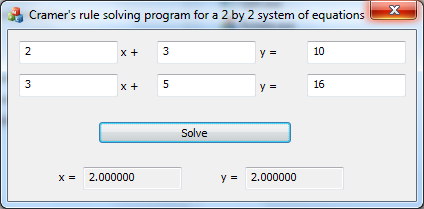
\includegraphics{Cramers}
\\

% Question 4
\item Dot product of A(2i + 3j + 5k) and B(-i + 7j + k) is
\[
2 \cdot {^-}1 + 3 \cdot 7 + 5 \cdot 1 = -2 + 21 + 5 = 24
\]

% Question 5
\item Angle between the vectors
\[
\underline{a}\cdot \underline{b} = \left| a \right| \left| b \right| cos \theta
\]

So
\[
24 = \sqrt{2^2 + 3^2 + 5^2} \sqrt{1^2 + 7^2 + 1^2} cos \theta = \sqrt{38} \sqrt{51} cos \theta \approx 44.023 cos \theta
\]

thus
\[
cos \theta \approx 0.545
\]

Therefore, to the nearest degree, the angle between the vectors is \[57{^\circ} \]

% Question 6
\item The vector equation of a line is
\[
\underline{r} = \underline{a} + \lambda(\underline{b} - \underline{a})
\]

So for this line
\[
\underline{r} = 2i + 3j + 5k + \lambda(-1i + 7j +k - 2i - 3j - 5k)
\]

Therefore
\[
\underline{r} = 2i + 3j + 5k + \lambda(-3i + 4j - 4k)
\]

%Question 7
\item Program for rotating point about origin \\
Please see Rotate.exe \\
The source code of most interest is Q7/RotateDlg.cpp from line 97. \\
\\
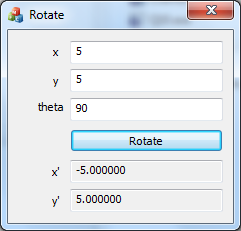
\includegraphics{Rotate}
\\

%Question 8
\item 3rd degree Lagrange Interpolant
\begin{multline}
P(x) = \frac{(x - x_2)(x - x_3)(x - x_4)}{(x_1-x_2)(x_1-x_3)(x_1-x_4)}y_1
        + \frac{(x - x_1)(x - x_3)(x - x_4)}{(x_2-x_1)(x_2-x_3)(x_2-x_4)}y_2 \\
        + \frac{(x - x_1)(x - x_2)(x - x_4)}{(x_3-x_1)(x_3-x_2)(x_3-x_4)}y_3
        + \frac{(x - x_1)(x - x_2)(x - x_3)}{(x_4-x_1)(x_4-x_2)(x_4-x_3)}y_4
\notag
\end{multline}

Passing through the points (-2,4), (-1,1), (1,1) and (2,4)
\begin{multline}
P(x) = \frac{(x - {^-}1)(x - 1)(x - 2)}{(-2-{^-}1)(-2-1)(-2-2)}4
        + \frac{(x -  {^-}2)(x - 1)(x - 2)}{( {^-}1- {^-}2)( {^-}1- 1)( {^-}1-2)}1 \\
        + \frac{(x - {^-}2)(x - {^-}1)(x - 2)}{(1-{^-}2)(1-{^-}1)(1-2)}1
        + \frac{(x - {^-}2)(x - {^-}1)(x -1)}{(2-{^-}2)(2-{^-}1)(2-1)}4
\notag
\end{multline}

\begin{multline}
P(x) = \frac{(x + 1)(x - 1)(x - 2)}{(1)(-3)(-4)}4
        + \frac{(x + 2)(x - 1)(x - 2)}{( 1)(-2)(-3)} \\
        + \frac{(x + 2)(x + 1)(x - 2)}{(3)(2)(-1)}
        + \frac{(x + 2)(x + 1)(x -1)}{(4)(3)(1)}4
\notag
\end{multline}

\begin{multline}
P(x) = \frac{(x + 1)(x - 1)(x - 2)}{3}
        + \frac{(x + 2)(x - 1)(x - 2)}{6} \\
        - \frac{(x + 2)(x + 1)(x - 2)}{6}
        + \frac{(x + 2)(x + 1)(x -1)}{3}
\notag
\end{multline}

%Question 9
\item Cubic Bezier:
\[
x = x_1(1-t)^3 + 3x_{c1}(1-t)^2t + 3x_{c2}(1-t)t^2 + x_2t^3
\]
\[
y = y_1(1-t)^3 + 3y_{c1}(1-t)^2t + 3y_{c2}(1-t)t^2 + y_2t^3
\]

Passing through (1,2) and (3,4)
\[
x = (1-t)^3 + 3x_{c1}(1-t)^2t + 3x_{c2}(1-t)t^2 + 3t^3
\]
\[
y = 2(1-t)^3 + 3y_{c1}(1-t)^2t + 3y_{c2}(1-t)t^2 + 4t^3
\]

%Question 10
\item Implement a cubic Bezier curve. \\
Please see Q10.exe \\
The source code of most interest is Q10/Q10.pde from line 83.
\\
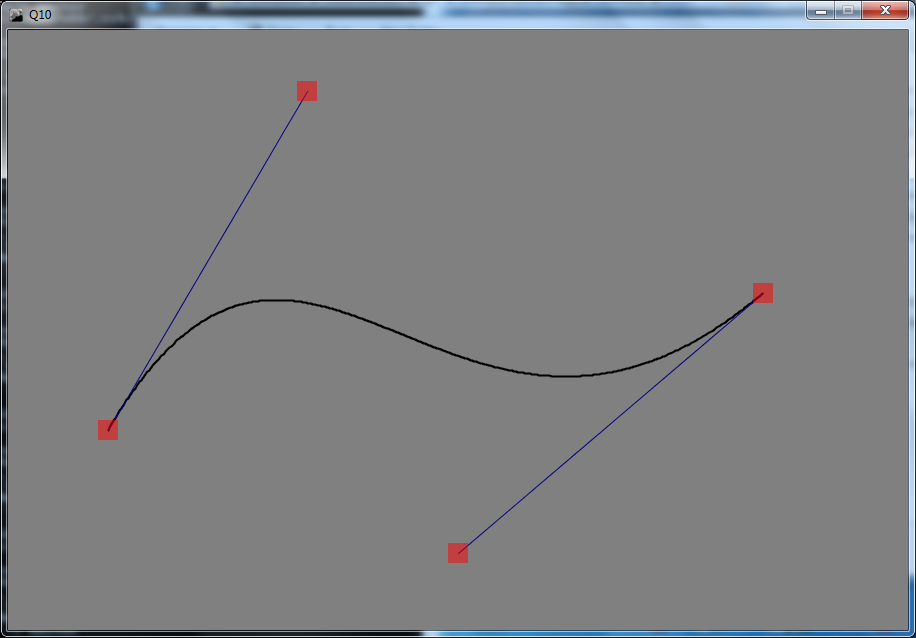
\includegraphics[scale=0.5]{Bezier}
\\

\end{enumerate}
\end{document}
